\section{Universe and news coverage}\label{app:universe}
Table~\ref{tab:universe} lists the firms with their accepted headlines for October 2010--December 2025; Figure~\ref{fig:coverage} shows the average number of headlines per firm and week by sector and year.
\begin{table}[p]\centering\tiny\setlength{\tabcolsep}{3pt}\renewcommand{\arraystretch}{0.92}\begin{tabular}{llrllr}
\toprule
Ticker & Company & Headlines & Ticker & Company & Headlines \\
\midrule
BMW.DE & BMW & 16,585 & COP & ConocoPhillips & 957 \\
ITX.MC & Inditex & 856 & CVX & Chevron & 3,815 \\
MBG.DE & Daimler (Mercedes-Benz Group) & 4,070 & DVN & Devon Energy & 260 \\
MC.PA & LVMH & 4,321 & HAL & Halliburton & 1,255 \\
VIV.PA & Vivendi & 468 & NOV & National Oilwell Varco & 89 \\
VOW3.DE & Volkswagen & 16,019 & OXY & Occidental Petroleum & 1,291 \\
ABI.BR & Anheuser-Busch InBev & 3,395 & SLB & Schlumberger & 1,936 \\
BN.PA & Danone & 2,057 & XOM & Exxon Mobil & 3,949 \\
CA.PA & Carrefour & 2,226 & AIG & American International Group & 3,362 \\
OR.PA & L'Oreal & 6,314 & ALL & Allstate & 1,912 \\
ULVR.L & Unilever & 6,547 & AXP & American Express & 6,054 \\
ENI.MI & Eni & 2,009 & BAC & Bank of America & 7,448 \\
REP.MC & Repsol & 1,394 & BK & Bank of New York Mellon & 1,475 \\
TTE.PA & Total (TotalEnergies) & 4,271 & BRK-B & Berkshire Hathaway & 3,304 \\
ALV.DE & Allianz & 2,134 & C & Citigroup & 6,899 \\
BBVA.MC & BBVA & 2,110 & COF & Capital One & 4,181 \\
BNP.PA & BNP Paribas & 2,844 & GS & Goldman Sachs & 9,534 \\
CS.PA & AXA & 2,032 & JPM & JPMorgan Chase & 8,863 \\
DBK.DE & Deutsche Bank & 4,626 & MET & MetLife & 3,251 \\
G.MI & Generali & 803 & MS & Morgan Stanley & 5,510 \\
GLE.PA & Societe Generale & 1,114 & SPG & Simon Property Group & 252 \\
INGA.AS & ING Groep & 390 & USB & U.S. Bancorp & 3,685 \\
ISP.MI & Intesa Sanpaolo & 455 & WFC & Wells Fargo & 7,817 \\
MUV2.DE & Munich Re & 815 & ABBV & AbbVie & 2,015 \\
SAN.MC & Banco Santander & 2,607 & ABT & Abbott Laboratories & 2,653 \\
UCG.MI & UniCredit & 935 & AMGN & Amgen & 1,964 \\
BAYN.DE & Bayer & 2,756 & BAX & Baxter International & 1,692 \\
EL.PA & Essilor (EssilorLuxottica) & 284 & BIIB & Biogen & 1,378 \\
SAN.PA & Sanofi & 3,112 & BMY & Bristol-Myers Squibb & 1,219 \\
AIR.PA & Airbus & 11,915 & GILD & Gilead Sciences & 2,642 \\
DG.PA & Vinci & 757 & JNJ & Johnson \& Johnson & 6,174 \\
DHL.DE & Deutsche Post DHL & 5,565 & LLY & Eli Lilly & 4,391 \\
PHIA.AS & Philips & 2,641 & MDT & Medtronic & 3,135 \\
SGO.PA & Saint-Gobain & 775 & MRK & Merck \& Co. & 3,991 \\
SIE.DE & Siemens & 8,343 & PFE & Pfizer & 6,621 \\
SU.PA & Schneider Electric & 2,080 & UNH & UnitedHealth Group & 1,720 \\
ASML.AS & ASML & 1,640 & BA & Boeing & 15,084 \\
NOKIA.HE & Nokia & 10,317 & CAT & Caterpillar & 2,539 \\
SAP.DE & SAP & 3,384 & EMR & Emerson Electric & 245 \\
AI.PA & Air Liquide & 584 & FDX & FedEx & 9,757 \\
BAS.DE & BASF & 2,041 & GD & General Dynamics & 1,542 \\
DTE.DE & Deutsche Telekom & 624 & GE & General Electric & 6,682 \\
ORA.PA & Orange & 70 & HON & Honeywell & 4,170 \\
TEF.MC & Telefonica & 1,130 & LMT & Lockheed Martin & 8,471 \\
ENEL.MI & Enel & 794 & MMM & 3M & 2,017 \\
ENGI.PA & GDF Suez (Engie) & 999 & NSC & Norfolk Southern & 1,595 \\
EOAN.DE & E.ON & 575 & RTX & United Technologies (RTX) & 468 \\
IBE.MC & Iberdrola & 943 & UNP & Union Pacific & 2,180 \\
RWE.DE & RWE & 1,099 & UPS & United Parcel Service & 3,417 \\
AMZN & Amazon.com & 7,347 & AAPL & Apple & 15,758 \\
CMCSA & Comcast & 6,589 & ACN & Accenture & 5,115 \\
DIS & Walt Disney & 15,723 & CSCO & Cisco Systems & 7,165 \\
F & Ford Motor & 6,189 & EBAY & eBay & 12,534 \\
GM & General Motors & 8,799 & GOOGL & Google (Alphabet) & 13,809 \\
HD & Home Depot & 6,777 & HPQ & Hewlett-Packard (HP Inc) & 1,182 \\
LOW & Lowe's & 3,021 & IBM & IBM & 9,164 \\
MCD & McDonald's & 15,468 & INTC & Intel & 14,687 \\
NKE & Nike & 6,195 & MA & Mastercard & 6,149 \\
SBUX & Starbucks & 14,342 & META & Facebook (Meta Platforms) & 16,273 \\
TGT & Target & 6,184 & MSFT & Microsoft & 12,010 \\
CL & Colgate-Palmolive & 818 & ORCL & Oracle & 5,346 \\
COST & Costco & 10,795 & QCOM & Qualcomm & 6,955 \\
CVS & CVS Health & 7,747 & TXN & Texas Instruments & 800 \\
KO & Coca-Cola & 13,440 & V & Visa & 1,794 \\
MDLZ & Mondelez International & 2,436 & DD & DuPont & 4,819 \\
MO & Altria & 716 & FCX & Freeport-McMoRan & 436 \\
PEP & PepsiCo & 11,284 & T & AT\&T & 11,195 \\
PG & Procter \& Gamble & 4,939 & VZ & Verizon & 10,460 \\
PM & Philip Morris International & 1,825 & EXC & Exelon & 437 \\
WMT & Walmart & 16,087 & SO & Southern Company & 404 \\
APA & Apache & 87 &  &  &  \\
\bottomrule
\end{tabular}

\caption{Research universe: members of the S\&P~100 and EURO STOXX~50 on 31 December 2014 with usable price histories, and their accepted headlines.}\label{tab:universe}\end{table}
\begin{figure}[H]\centering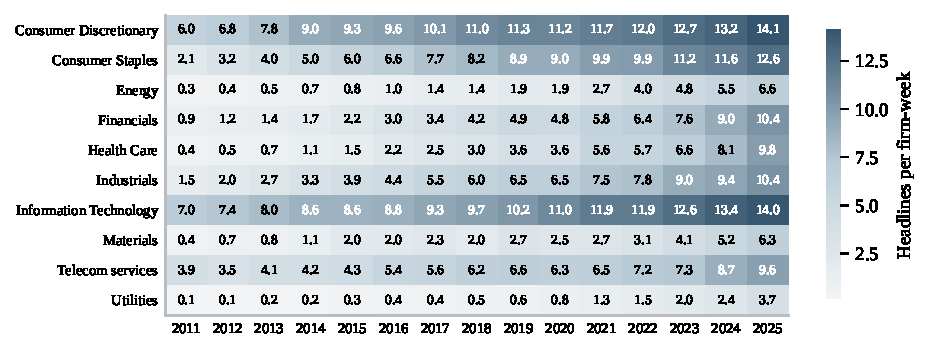
\includegraphics[width=\textwidth]{coverage}
\caption{Accepted headlines per firm and week, by sector and year.}\label{fig:coverage}\end{figure}

\section{Drawdowns and annual returns}\label{app:annual}
\begin{figure}[H]\centering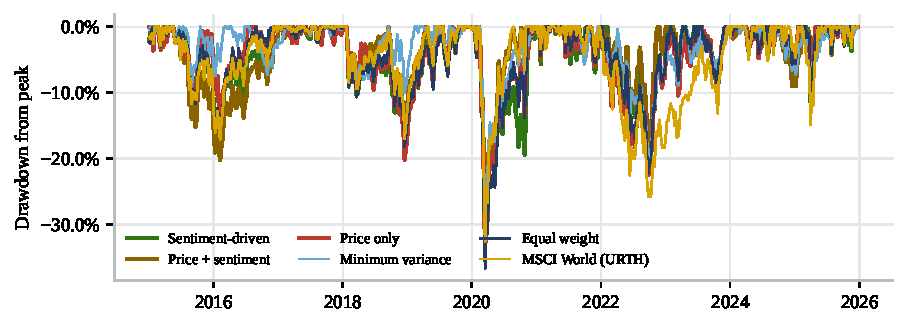
\includegraphics[width=\textwidth]{drawdown}
\caption{Drawdown from the previous peak after costs, 2015--2025.}\label{fig:drawdown}\end{figure}
\begin{figure}[H]\centering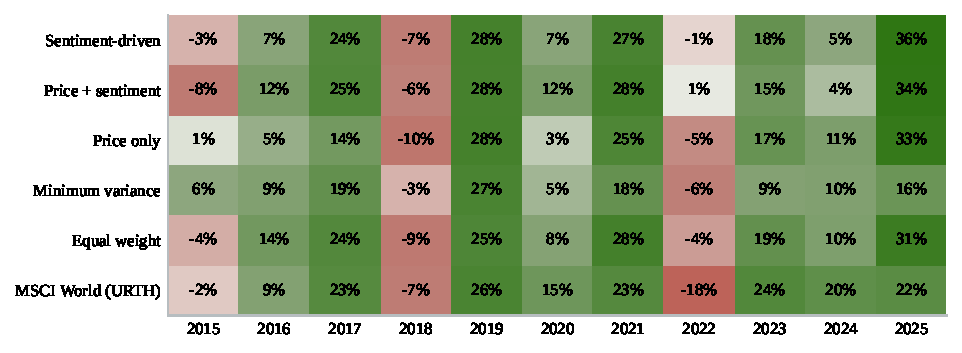
\includegraphics[width=\textwidth]{annual}
\caption{Net annual returns by strategy and year.}\label{fig:annual}\end{figure}

\section{Reproduction}\label{app:code}
{\sloppy All results, tables and figures are produced from the stored data by \texttt{project.py} in four stages: \texttt{validate-price} and \texttt{validate-sentiment} (2012--2014 only), \texttt{freeze}, which stores a SHA-256 fingerprint of the code, settings and validation choices, and \texttt{test}, which refuses to run if anything changed after freezing and runs only once. Package versions and input file hashes are recorded in \texttt{results/test\_run.json}.\par}
